\documentclass[10pt,twocolumn,letterpaper]{article}

\usepackage{statcourse}
\usepackage{times}
\usepackage{epsfig}
\usepackage{graphicx}
\usepackage{amsmath}
\usepackage{amssymb}

% Include other packages here, before hyperref.

% If you comment hyperref and then uncomment it, you should delete
% egpaper.aux before re-running latex.  (Or just hit 'q' on the first latex
% run, let it finish, and you should be clear).
\usepackage[breaklinks=true,bookmarks=false]{hyperref}


\statcoursefinalcopy


\setcounter{page}{1}
\begin{document}


%%%%%%%%%%%%%%%%%%%%%%%%%%%%%%%%%%%%%%%%%%%%%%%%%%%%%%%%%%%%%%%
% DO NOT EDIT ANYTHING ABOVE THIS LINE
% EXCEPT IF YOU LIKE TO USE ADDITIONAL PACKAGES
%%%%%%%%%%%%%%%%%%%%%%%%%%%%%%%%%%%%%%%%%%%%%%%%%%%%%%%%%%%%%%%



%%%%%%%%% TITLE
\title{\LaTeX\ Template for Project Proposal (\textit{replace with your project title})}

\author{First Author\\
{\tt\small firstauthor@wisc.edu}
\and
Second Author\\
{\tt\small secondauthor@wisc.edu}
\and
Third Author\\
{\tt\small thirdauthor@wisc.edu}
}

\maketitle
%\thispagestyle{empty}



% MAIN ARTICLE GOES BELOW
%%%%%%%%%%%%%%%%%%%%%%%%%%%%%%%%%%%%%%%%%%%%%%%%%%%%%%%%%%%%%%%



%%%%%%%%% BODY TEXT



\begin{itemize}


	\item The information in this template is very minimal, and this file should serve you as a framework for writing your proposal. You may prefer to use a more collaboration-friendly tool while drafting the report with your classmates before you prepare the final report for submission. Remember that you only need to turn in the PDF file on Canvas. Also, \textbf{only one member per team} needs to submit the project proposal.
	
	\item The project proposal is a 2-3 page document excluding references\footnote{This means, references should of course be included but do not count towards the page limit}.
	
	\item You are encouraged (not required) to use 1-2 figures to illustrate technical concepts.
	
	\item The proposal must be formatted and submitted as a PDF document on Canvas (the submission deadline will be later announced on Canvas.
	
	\item Please
	check out the text in the sections below for further information.
	
\end{itemize}




\section{Introduction}


In this section, describe what you are planning to do. Also, briefly describe related work.

\subsection{Notes about Citations}

When discussing related work, do not forget to include appropriate references.  This is an example of a citation \cite{paszke2019pytorch}. To format the citations properly, put the
corresponding references into the ``bibliography.bib`` file. You can obtain
BibTeX-formatted references for the "bib" file from Google Scholar 
(\url{https://scholar.google.com}), for example, by clicking on the 
double-quote character under a citation and then selecting \mbox{"BibTeX"} as
shown in Figure \ref{fig:google-scholar-1col} and 
Figure \ref{fig:google-scholar-2col}.

To avoid plagiarism, any sentence that is copied from other articles or sources (internet, papers, etc.) must be put in quotation marks. The next sentence provides and example that uses an existing sentence verbatim. 

According to \cite{Raschka2020PythonTrends}, "The development of machine learning algorithms that operate on a set of values (as opposed to a single value) at a time is also commonly known as vectorization." 

Direct quotes should be used sparingly, and it is usually better to rephrase sentences in your own words.  The next sentence provides an example.

Vectorization is a programming approach utilizing functions that operate on multiple values simultaneously to speed up computation \cite{Raschka2020PythonTrends}.

\begin{figure}[t]
\begin{center}
   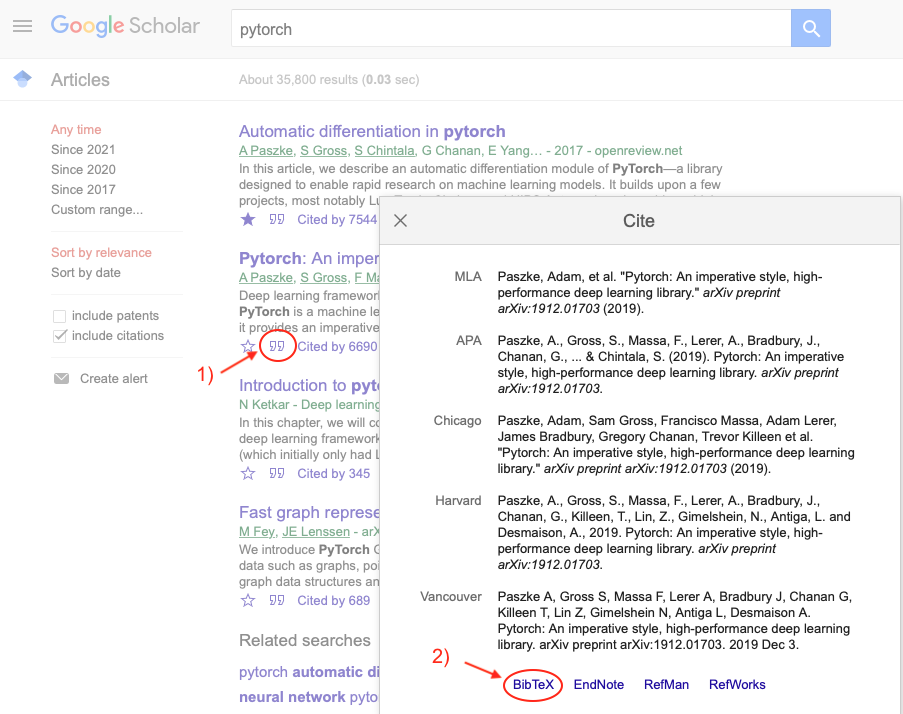
\includegraphics[width=0.8\linewidth]{figures/google-scholar.png}
\end{center}
   \caption{Example illustrating how to get BibTeX references from
   Google Scholar as a 1-column figure.}
\label{fig:google-scholar-1col}
\end{figure}

\subsection{Notes about Figures}

Figure~\ref{fig:google-scholar-1col} shows an example of a 1-column figures.

You can create two-column figures, too, as shown in Figure \ref{fig:google-scholar-2col}. Please not that you can reuse figures from other papers or lecture material, but for every figure that is not your own, you have to include the "Source" as shown in Figure~\ref{fig:other-figure}.

\begin{figure*}
\begin{center}
   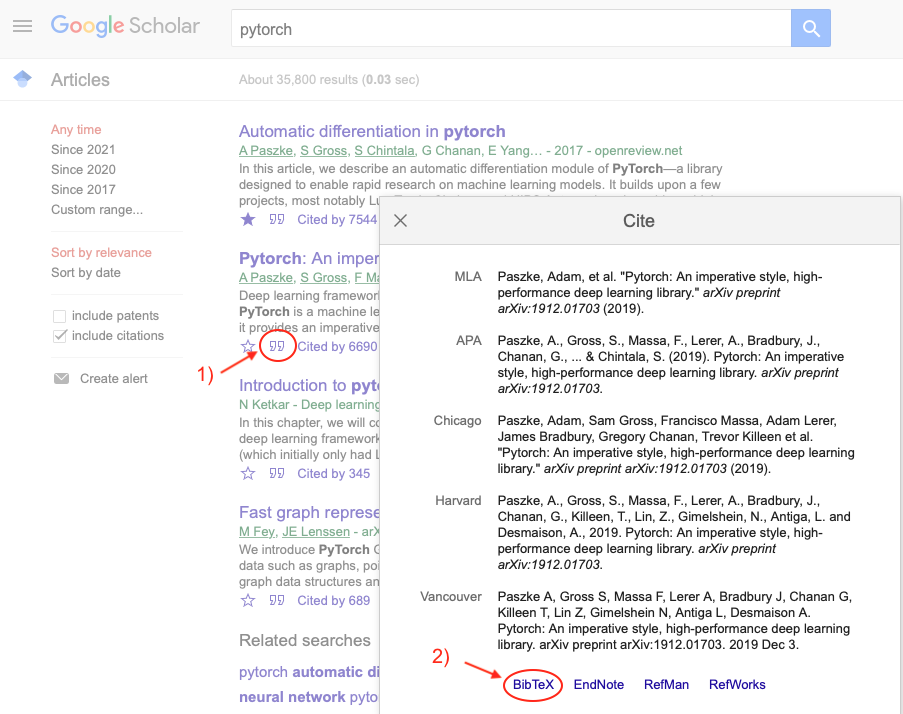
\includegraphics[width=0.8\linewidth]{figures/google-scholar.png}
\end{center}
   \caption{Example of a 2-column figure.}
\label{fig:google-scholar-2col}
\end{figure*}

\begin{figure*}
\begin{center}
   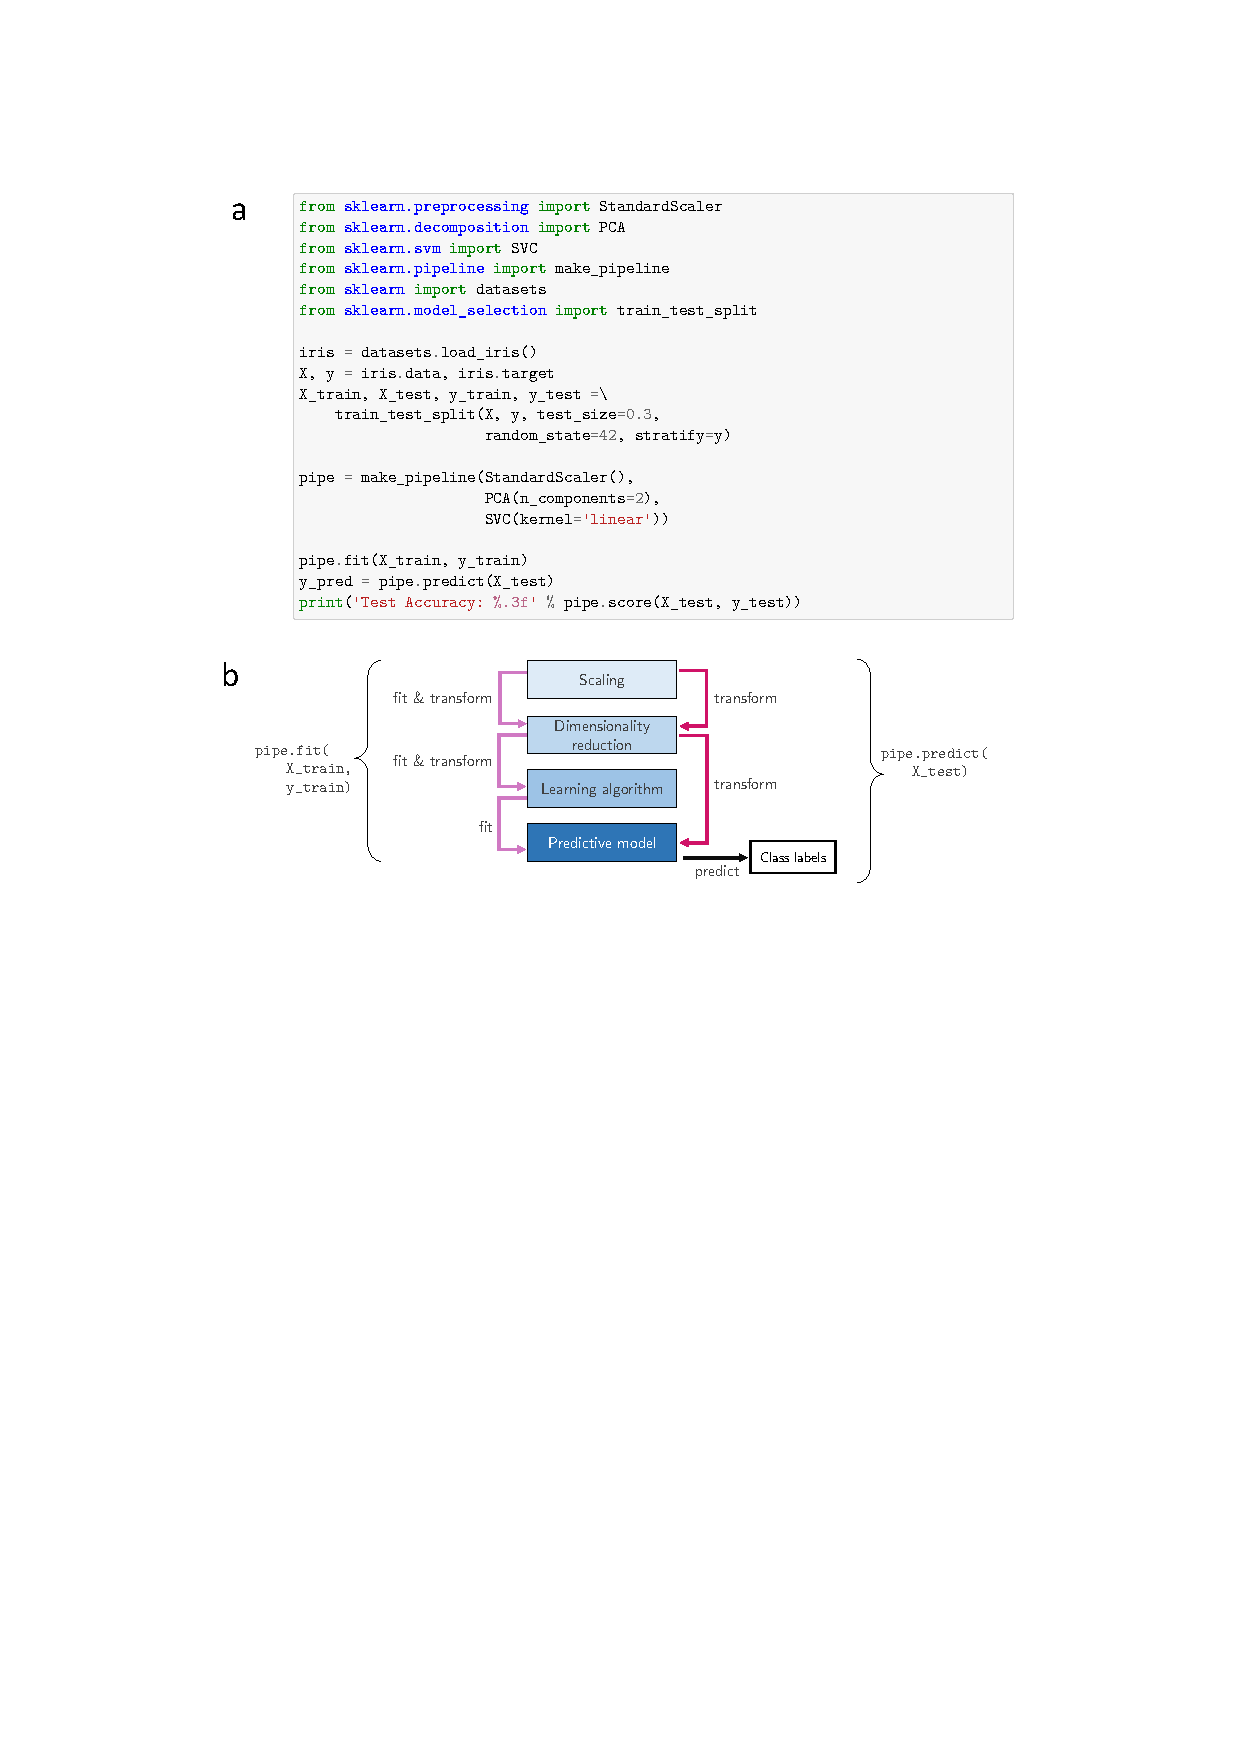
\includegraphics[width=0.8\linewidth]{figures/not-own-figure.pdf}
\end{center}
   \caption{Figure note created by yourself. Image source: \cite{Raschka2020PythonTrends}. (If the source is a website, not a paper, please use the URL link instead of the paper reference. Image source: \url{https://www.mdpi.com/2078-2489/11/4/193}.)}
\label{fig:other-figure}
\end{figure*}


\section{Motivation}

Describe why your project is interesting. E.g., you can describe why your project could have a broader societal impact. Or, you may describe the motivation from a personal learning perspective.

\section{Evaluation}

What would the successful outcome of your project look like? In other words, under which circumstances would you consider your project to be “successful?”

How do you measure success, specific to this project, from a technical standpoint?

\section{Resources}

Describe what resources you are planning to use (datasets, computer hardware, computational tools, etc.)?

\section{Contributions}

You are expected to share the workload evenly, and every group member is expected to participate in both the experiments and writing. (As a group, you only need to submit one proposal and one report, though. However, you will need to work together and coordinate your efforts.)

Clearly indicate what computational and writing tasks each member of your group will be participating in.


{\small
\bibliographystyle{ieee}
\bibliography{bibliography.bib}
}

\end{document}
